%!TeX root=../tese.tex
%("dica" para o editor de texto: este arquivo é parte de um documento maior)
% para saber mais: https://tex.stackexchange.com/q/78101

\chapter{Resultados}
\label{chap:resultados}

No capítulo \ref{chap:experimentos}, foram realizados experimentos para encontrar a combinação de 
parâmetros que proporcionava melhor desempenho para as categorias de modelos 
testadas neste estudo, regressão linear, redes \textit{feed forward}, redes
recorrentes e redes bidirecionais. Neste capítulo, são apresentadas as previsões 
dos diferentes modelos.

É possível comparar o desempenho dos modelos a partir da tabela \ref{tab:compara_modelos}:

\begin{table}[H]
    \centering
    \begin{tabular}{llll}
        \toprule
        Modelo & MAE     & RMSE    & MAPE \\
        \midrule
        Regressão linear & 26435 & 38970 & 0.32  \\
        Rede \textit{feed forward} & 26880  & 50830 & 0.27 \\
        Rede recorrente & 22694 & 43918 & 0.19  \\
        \textbf{Rede bidirecional} & \textbf{19185} & \textbf{33942} & \textbf{0.17} \\
        \bottomrule
    \end{tabular}
    \caption{Comparação do desempenho dos modelos}
    \label{tab:compara_modelos}
\end{table}

Na análise da tabela acima, nota-se que o desempenho nas previsões
melhora à medida que se aumenta a robustez do modelo. A regressão linear é utilizada 
como base para avaliar o desempenho das redes neurais por ser um modelo mais 
simples. 

É possível perceber que houve uma ligeira melhora das previsões com as 
redes \textit{feed forward} em relação à regressão linear que se refletiu na 
redução do erro médio percentual
em 5\%. Essa melhora, contudo, não é perceptível nos indicadores de erro absoluto,
enquanto a MAE apresenta um valor similar ao da regressão, a RMSE teve um 
aumento significativo, o que indica a presenta de \textit{outliers}.

Observa-se uma significativa melhora, de 8\%, das redes \textit{feed forward} para os modelos
de redes recorrentes, reflexo da capacidade de reconhecer sequências e contexto.
A melhora também se reflete nos erros absolutos calculados pela MAE, contudo, a 
RMSE apresentou piora em relação à regressão linear, provavelmente por conta 
de \textit{outliers}, uma vez que a RMSE é mais sensível a valores discrepantes.

As redes bidirecionais apresentaram melhor desempenho em comparação com os outros 
modelos, isso em virtude da arquitetura mais complexa com duas redes recorrentes. Percebeu-se também uma
redução de 2\% da MAPE em relação às redes recorrentes e de 15\% em relação à 
regressão linear. Esse comportamento também se reflete nos indicadores de 
erro absoluto que são os menores entre as classes de algoritmos testados.

No presente trabalho, foi adotado o estado de São Paulo como objeto de observação mais detalhado para comparar as previsões e o valor real 
do consumo, essa escolha foi tomada por 
se tratar do maior consumidor de cimento no Brasil\footnote{Em 2019, o estado 
de São Paulo foi 
responsável por 21.3\% da demanda por cimento no Brasil, 8.6\% à frente do 
segundo maior consumidor, Minas Gerais.}, de tal forma que a evolução do consumo 
mensal de cimento em São Paulo pode ser vista na figura \ref{consumo-sp}:

\begin{figure}[H]
    \centering
    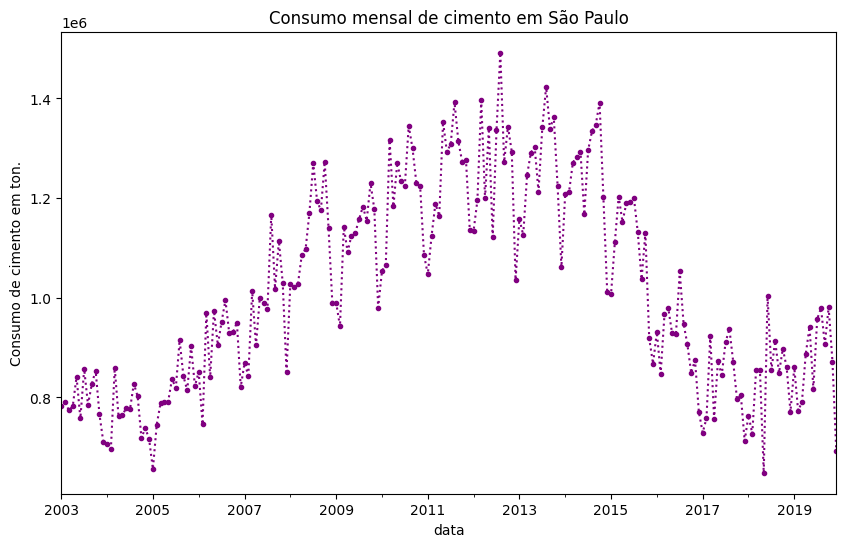
\includegraphics[width=11cm]{../figuras/graficos/evolucao-consumo-sp.png}
    \caption{Evolução do consumo mensal de cimento em São Paulo}
    \label{consumo-sp}
\end{figure}

Na imagem acima, os círculos representam as medições mensais do consumo de 
cimento em São Paulo. Observa-se que a demanda por cimento no estado vinha em tendência
de queda desde 2013 e passou a apresentar alta de 2018 em diante, além disso, há certa
sazonalidade da demanda.

Os modelos foram utilizados para prever o consumo mensal de 
cimento a partir de julho de 2017. Os gráficos do consumo real 
e da previsão realizada pelo modelo são sobrepostos para melhor
visualização. Nos gráficos das previsões apresentados neste 
capítulo, o consumo real está representado em azul claro e 
as previsões do modelo, em laranja, além disso, a linha 
tracejada em cinza marca julho de 2017, início das previsões.

\section{Regressão linear}

Comparou-se as previsões realizadas pela regressão linear com o valor real 
que foi demandado de cimento, tendo isso em mente, na imagem \ref{img:erro-perc-rg}, representa-se 
distribuição do erro percentual das previsões:

\begin{figure}[H]
    \centering
    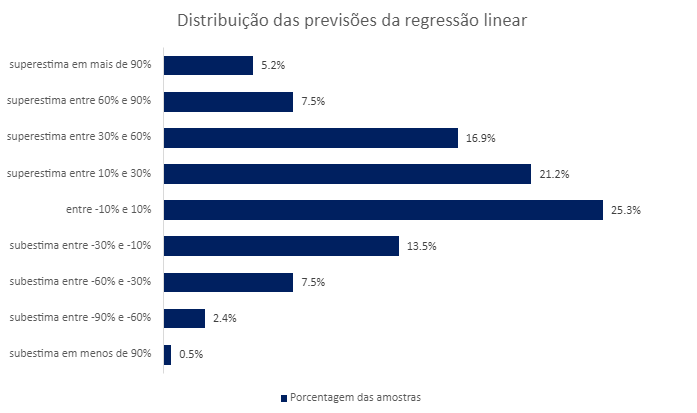
\includegraphics[width=10cm]{../figuras/graficos/reg_lin/erro-perc-rg.png}
    \caption{Distribuição da variação percentual das previsões da regressão linear}
    \label{img:erro-perc-rg}
\end{figure}

No gráfico acima, é possível ver que o modelo concentra 60\% das previsões 
com erro percentual menor ou igual a 30\%. Além disso, observa-se uma 
tendência de superestimar o valor do consumo, uma vez que 50.8\% das previsões
superestimam o valor real em mais de 10\%. 

As previsões realizadas pela regressão linear para o estado 
de São Paulo podem ser visualizadas na imagem \ref{prev-sp-rg}:

\begin{figure}[H]
    \centering
    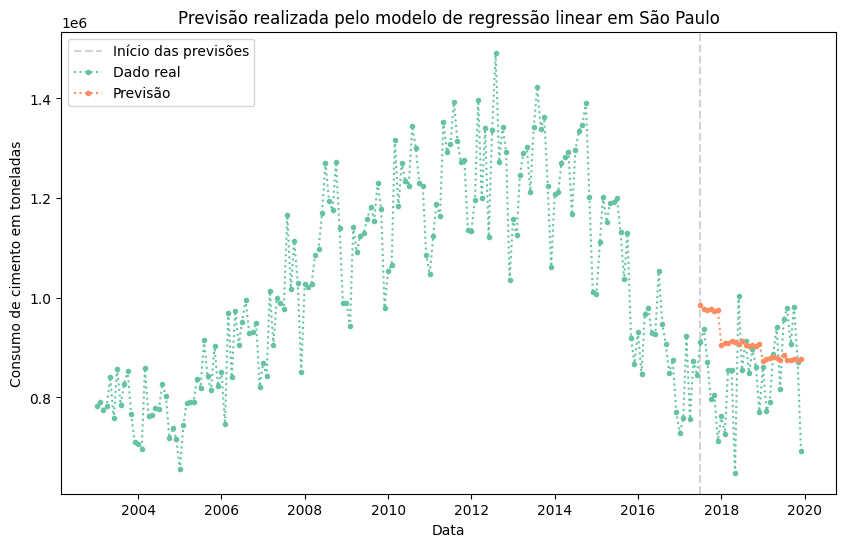
\includegraphics[width=10cm]{../figuras/graficos/reg_lin/prev_sp.png}
    \caption{Previsão realizada pela regressão linear para o 
    consumo de cimento em São Paulo}
    \label{prev-sp-rg}
\end{figure}

Destaca-se na figura \ref{prev-sp-rg} a proximidade das previsões realizadas 
ao longo dos meses de um ano, são perceptíveis variações apenas na passagem de um 
ano para o seguinte. Uma possível explicação para esse comportamento são as 
variáveis que originalmente possuíam granularidade anuais utilizadas como atributos.

Para o estado de São Paulo, as previsões estão com valores próximos aos
reais. Apesar disso, o modelo previu que a tendência de queda, presente
nos dados até 2018, continuaria em 2018 e 2019, contudo o consumo real passou 
a apresentar alta.

\section{Redes \textit{feed forward}}

As redes \textit{feed forward} são modelos mais robustos que a regressão linear.
A distribuição da diferença percentual entre as previsões e os valores reais 
do consumo é dada na figura \ref{img:erro-perc-rff}:

\begin{figure}[H]
    \centering
    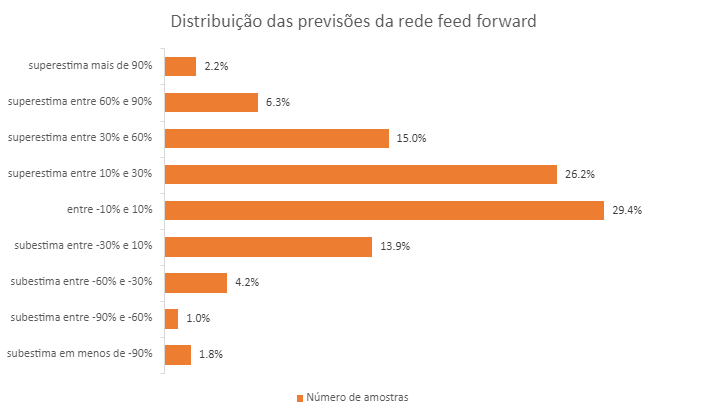
\includegraphics[width=10cm]{../figuras/graficos/mlp/erro-perc-mlp.png}
    \caption{Distribuição da variação percentual das previsões das redes \textit{feed forward}}
    \label{img:erro-perc-rff}
\end{figure}

Ao analisar o gráfico acima, observa-se que as redes \textit{feed forward}
concentram 69.5\% das previsões com erro percentual de até 30\%, dessa forma, 
há melhora de 9.5\% em comparação com a regressão linear. Essas redes ainda 
apresentam tendência a superestimar o consumo, contudo, em menor grau que 
a regressão linear, já que 49.7\% das previsões sobrestimam  o valor real 
em mais de 10\%.

Na imagem \ref{img:consumo-sp-rff}, são dadas as previsões do modelo para o estado 
de São Paulo:

\begin{figure}[H]
    \centering
    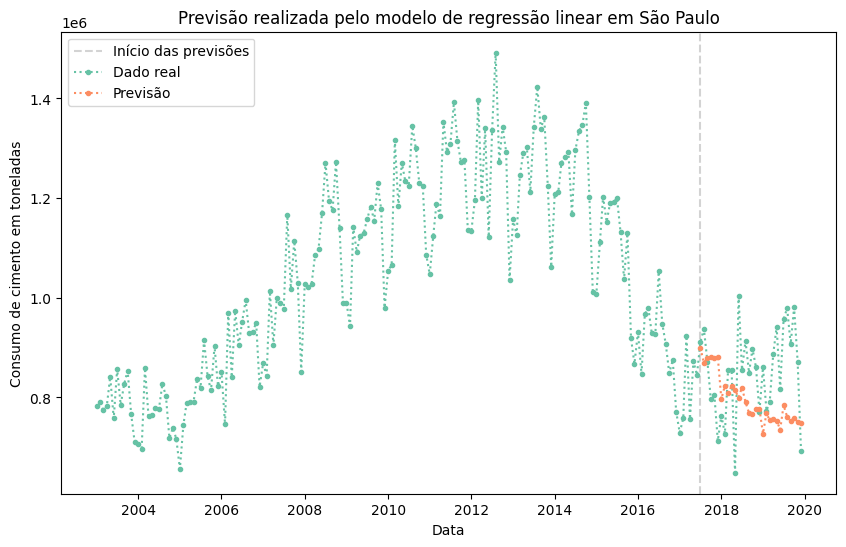
\includegraphics[width=10cm]{../figuras/graficos/mlp/prev_sp.png}
    \caption{Previsão realizada pelas redes \textit{feed forward} em São Paulo}
    \label{img:consumo-sp-rff}
\end{figure}

Observa-se na imagem que o modelo capturou a leve tendência de aumento do 
consumo a partir de 2018, contudo as previsões superestimam o valor real 
do consumo.

\section{Redes recorrentes}

A distribuição do erro percentual das previsões realizadas pelas redes 
recorrentes pode ser observada na figura \ref{img:erro-perc-rnn}:

\begin{figure}[H]
    \centering
    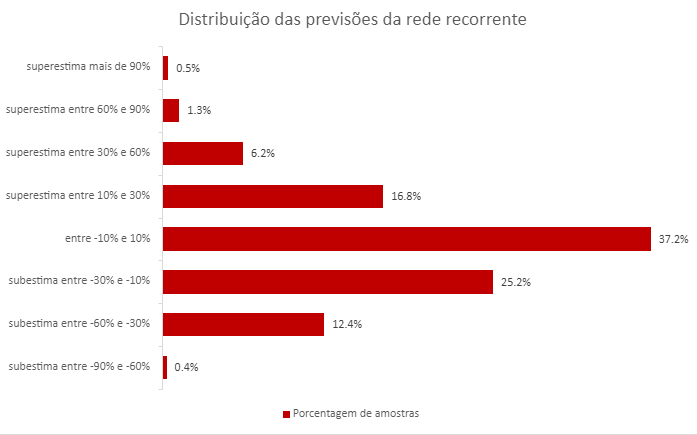
\includegraphics[width=10cm]{../figuras/graficos/rnn/erro-perc-rnn.png}
    \caption{Distribuição da variação percentual das previsões das redes recorrentes}
    \label{img:erro-perc-rnn}
\end{figure}

Na análise do gráfico acima, é perceptível o impacto da análise de contexto histórico 
nas previsões realizadas pelas redes recorrentes. As previsões com erro percentual 
de até 30\% correspondem a 79.2\% do conjunto de teste, um aumento de 9.7\% em 
relação à rede \textit{feed forward} e de 19.2\% em relação à regressão linear.
Além disso, destaca-se que 37.2\% das previsões apresentaram erro percentual 
de até 10\%. Inversamente à regressão linear e das redes \textit{feed forward},
as redes recorrentes apresentam tendência de subestimar o consumo, com 38\% das
previsões com valores subestimando o valor real do consumo em mais de 30\%.

Na figura \ref{img:consumo-sp-rnn}, é possível observar as previsões realizadas pelas 
redes recorrentes no estado de São Paulo:

\begin{figure}[H]
    \centering
    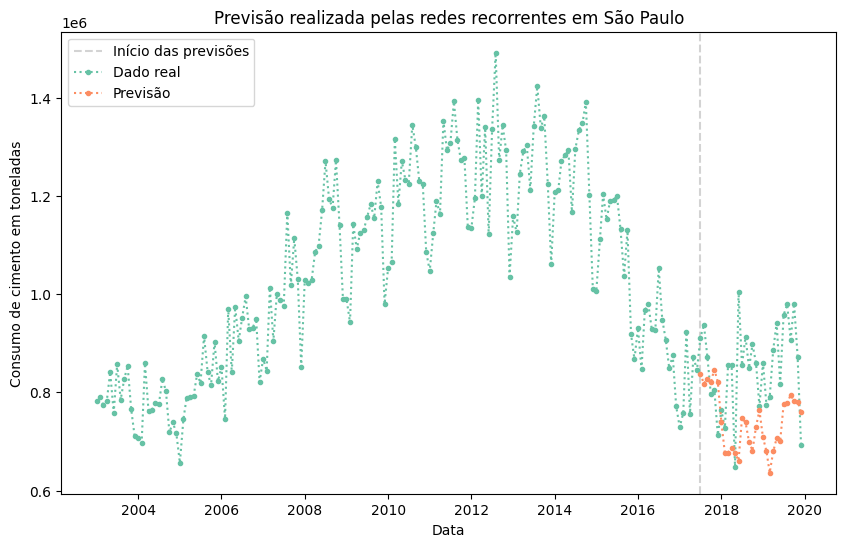
\includegraphics[width=10cm]{../figuras/graficos/rnn/prev_sp.png}
    \caption{Previsão realizada pelas redes recorrentes em São Paulo}
    \label{img:consumo-sp-rnn}
\end{figure}

Por meio do gráfico, é possível evidenciar que o modelo capturou com precisão a tendência do 
consumo, primeiro de queda até 2018 e aumento após essa data. Destaca-se, 
também, a proximidade das previsões realizadas pelas redes recorrentes e o 
valor real do consumo, embora o modelo tenha tendência de subestimar o valor.


\section{Redes bidirecionais}

Na imagem \ref{img:erro-perc-bnn}, está a distribuição do erro percentual das 
previsões realizadas ao utilizar redes bidirecionais:

\begin{figure}[H] 
    \centering
    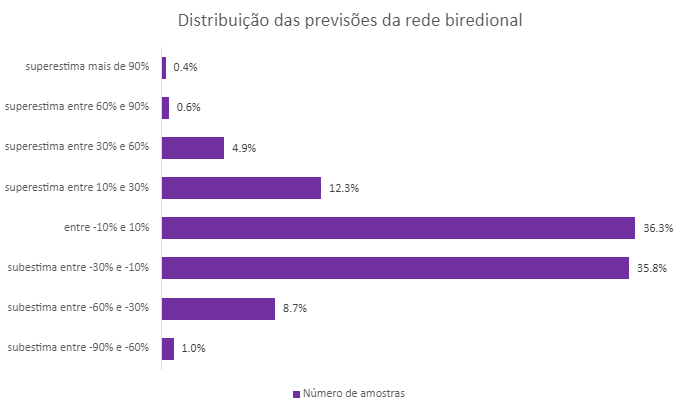
\includegraphics[width=10cm]{../figuras/graficos/bi/erro-perc-bi.png}
    \caption{Distribuição da variação percentual das previsões das redes bidirecionais}
    \label{img:erro-perc-bnn}
\end{figure}

Observa-se no gráfico acima, a melhora no desempenho ao utilizar a arquitetura 
robusta das redes bidirecionais: 84.4\% das previsões desse modelo apresentam 
erro de até 30\%, um crescimento de 5.2\% ao comparar com as redes recorrentes 
e de 24.4\% ao comparar com a regressão linear. Destaca-se, também, uma tendência
maior de subestimar o valor real, 45.5\%¨subestimam o consumo real em mais de 
30\%,

Na imagem \ref{img:consumo-sp-bnn}, encontram-se as previsões realizadas pelo 
modelo para São Paulo:

\begin{figure}[H]
    \centering
    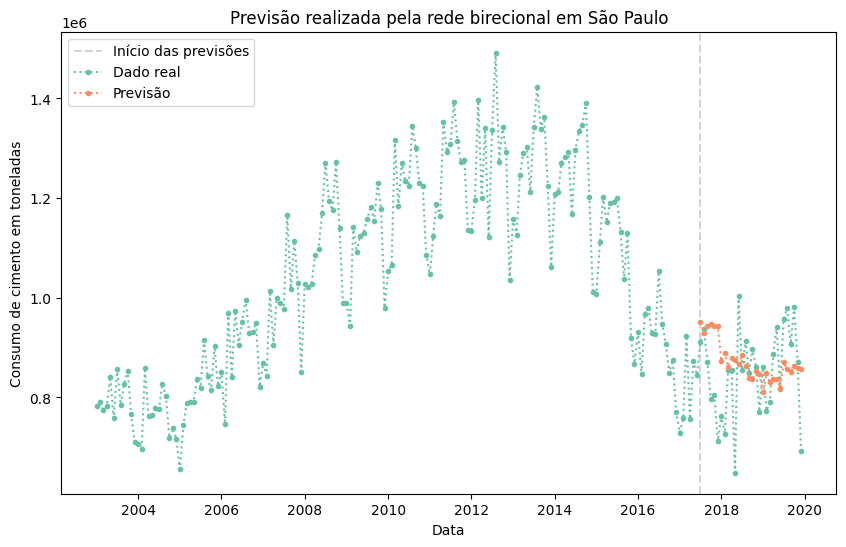
\includegraphics[width=10cm]{../figuras/graficos/bi/prev-sp-bi.png}
    \caption{Previsão realizada pelas redes bidirecionais em São Paulo}
    \label{img:consumo-sp-bnn}
\end{figure}

Destaca-se na figura acima a assertividade das previsões realizadas pelas 
redes bidirecionais. O modelo não apenas captura de forma certeira a tendência 
do consumo, como prevê valor muito próximos ao valor real. Por isso mesmo, em comparação com 
as previsões realizadas pelos outros modelos testados nesta trabalho, trata-se 
da previsão mais precisa.